\chapter{Results}  % Now \chapter will work

\section{Evaluation Metrics}

The models' performance is evaluated using the following metrics:

\begin{itemize}
    \item \textbf{Accuracy:} Measures the proportion of correctly classified instances out of the total instances.
    \item \textbf{Precision:} Measures the proportion of true positive instances out of the total predicted positive instances.
    \item \textbf{Recall:} Measures the proportion of true positive instances out of the total actual positive instances.
    \item \textbf{F1 Score:} The harmonic mean of precision and recall, providing a single metric that balances both.
\end{itemize}

The table below summarizes the evaluation metrics for the models:

\begin{table}[htbp]
  \centering
  \caption{Evaluation Metrics for the Models}
  \vspace{0.5cm}  % Adjust the space here if needed
  \begin{tabular}{@{\hskip 5pt} l @{\hskip 10pt} c @{\hskip 10pt} c @{\hskip 10pt} c @{\hskip 10pt} c @{\hskip 5pt}}
  \toprule
  \textbf{Model} & \textbf{Accuracy} & \textbf{Precision} & \textbf{Recall} & \textbf{F1 Score} \\
  \midrule
  VGG-16 Fine-tuned  & 0.997691 & 0.997712 & 0.997691 & 0.997691 \\
  VGG-16  & 0.993072 & 0.993093 & 0.993072 & 0.993072 \\
  CNN        & 0.969977 & 0.969997 & 0.969977 & 0.969977 \\
  \bottomrule
  \end{tabular}
\end{table}
\newpage % Forces the next section to start on a new page

\section{VGG-16 Fine-tuned}

\subsection{Training and Validation Loss}

\begin{figure}[htbp]
\centering
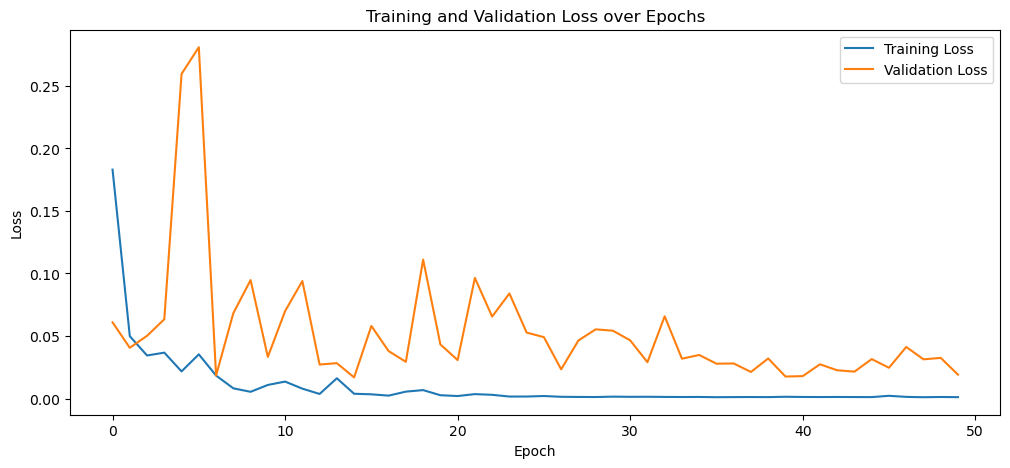
\includegraphics[width=0.8\textwidth]{train_val_loss_vgg16_uf.png}
\caption{Training and Validation Loss for VGG16 Fine-tuned (last 3 layers)}
\end{figure}

\subsection{Training and Validation Accuracy}

\begin{figure}[htbp]
\centering
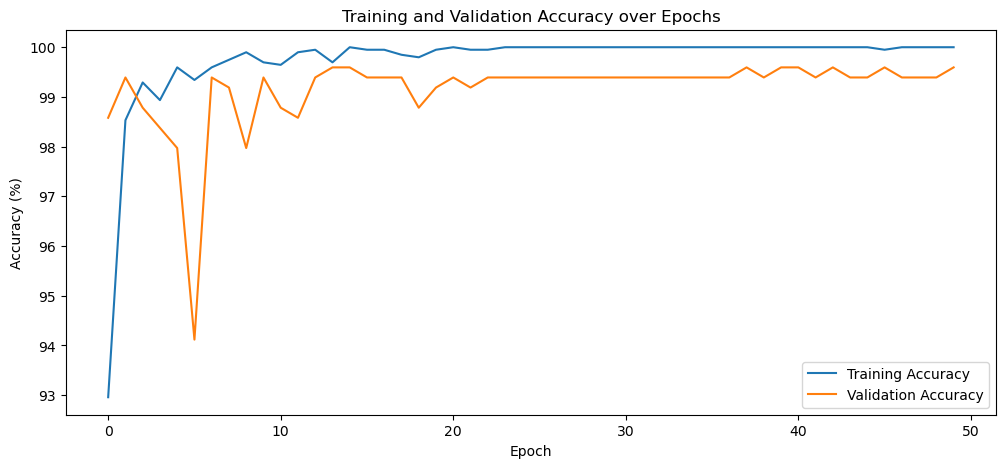
\includegraphics[width=0.8\textwidth]{train_val_acc_vgg16_uf.png}
\caption{Training and Validation Accuracy for VGG16 Fine-tuned (last 3 layers)}
\end{figure}

\newpage % Forces the next section to start on a new page

\section{VGG-16 with All Convolutional Layers Frozen}

\subsection{Training and Validation Loss}

\begin{figure}[htbp]
\centering
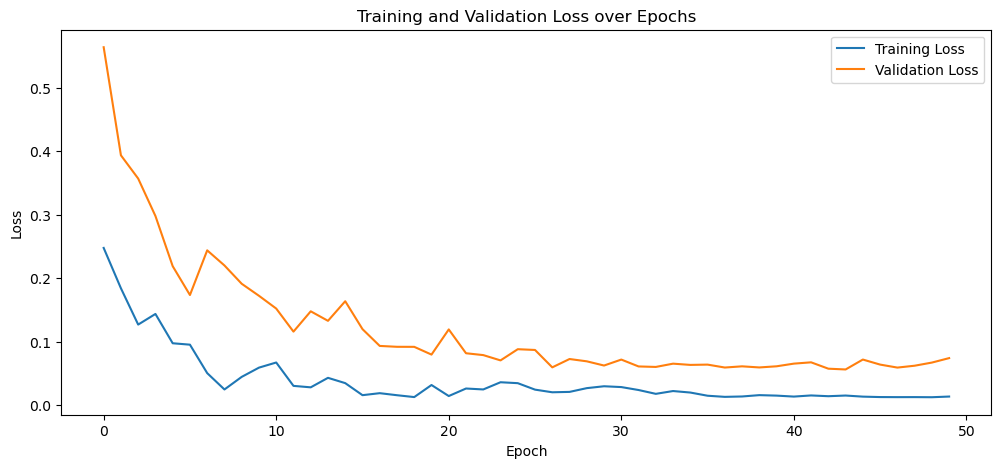
\includegraphics[width=0.8\textwidth]{train_val_err_vgg16.png}
\caption{Training and Validation Loss for VGG16 with Learning Rate Scheduler}
\end{figure}

\subsection{Training and Validation Accuracy}

\begin{figure}[htbp]
\centering
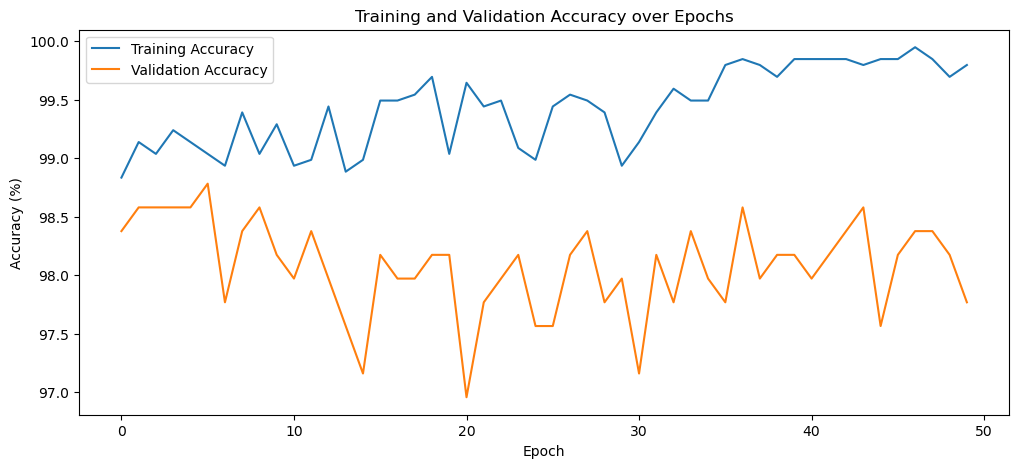
\includegraphics[width=0.8\textwidth]{train_val_acc_vgg16.png}
\caption{Training and Validation Accuracy for VGG16 with Learning Rate Scheduler}
\end{figure}

\newpage % Forces the next section to start on a new page

\section{Lightweight CNN}

\subsection{Training and Validation Loss}

\begin{figure}[htbp]
\centering
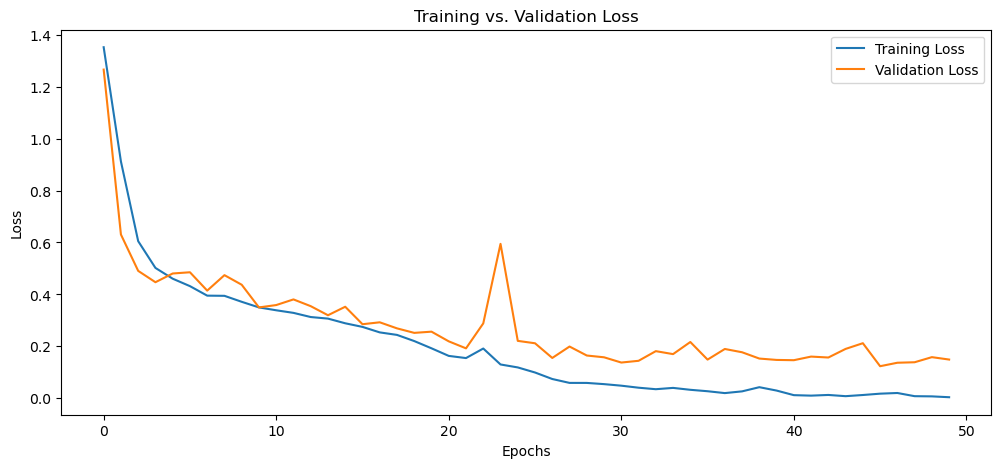
\includegraphics[width=0.8\textwidth]{train_valid_err_cnn.png}
\caption{Training and Validation Loss for Lightweight CNN}
\end{figure}

\subsection{Training and Validation Accuracy}

\begin{figure}[htbp]
\centering
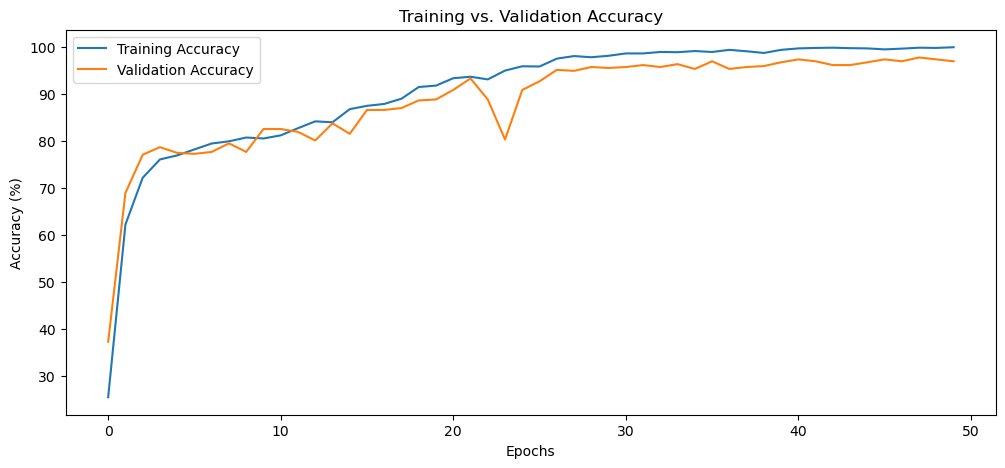
\includegraphics[width=0.8\textwidth]{train_valid_acc_cnn.png}
\caption{Training and Validation Accuracy for Lightweight CNN}
\end{figure}

\newpage % Forces the next section to start on a new page

\section{Confusion Matrix}

\begin{figure}[htbp]
\centering
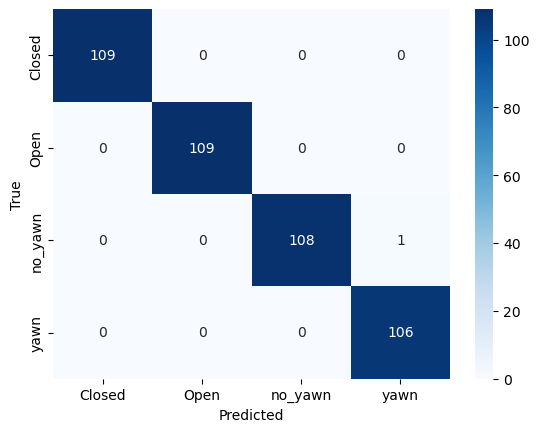
\includegraphics[width=0.8\textwidth]{vgg_16_unfreeze.png}
\caption{Confusion Matrix for VGG16 with Last 3 Convolutional Layers Unfrozen}
\end{figure}

\begin{figure}[htbp]
\centering
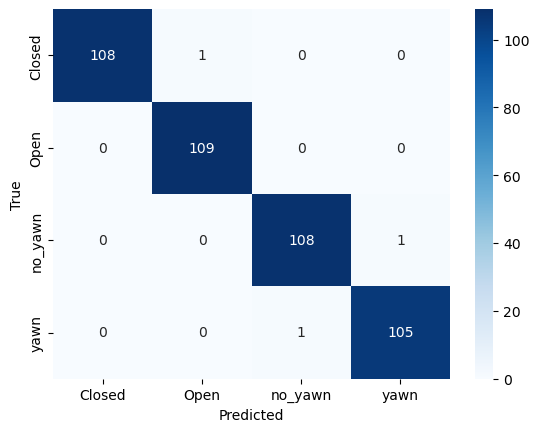
\includegraphics[width=0.8\textwidth]{vgg_16_freeze.png}
\caption{Confusion Matrix for VGG16 with All Convolutional Layers Frozen}
\end{figure}

\begin{figure}[htbp]
\centering
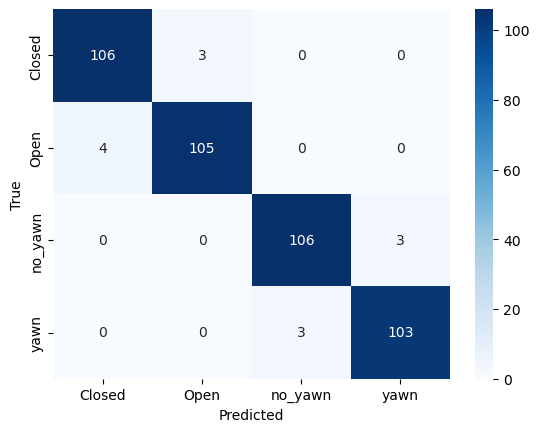
\includegraphics[width=0.8\textwidth]{conf_cnn.png}
\caption{Confusion Matrix for Lightweight CNN}
\end{figure}
